\section{Administración final del proyecto}

\subsection{Backlog final}
El backlog final tiene 21 requerimientos funcionales (RF-01 a RF-21), 36 historias de usuario en 8 épicas (E1 Acceso y perfiles a E8 Confiabilidad y trazabilidad), tareas técnicas y requerimientos no funcionales. Los RNF de seguridad agregados en esta entrega son RNF-SEG-01 a 08 y RNF-PRIV-01 (sección~\ref{sec:estado}). El tablero se administra en Microsoft Planner:

\begin{itemize}
	\item Plan de Planner: \href{https://teams.microsoft.com/l/entity/com.microsoft.teamspace.tab.planner/_djb2_msteams_prefix_3923924113?context=\%7B\%22channelId\%22\%3A\%2219\%3A17zu_w8a-xo5ieToH61foRRfCKvnOu6HKuCw9bj4xts1\%40thread.tacv2\%22\%7D&tenantId=c65a3ea6-0f7c-400b-8934-5a6dc1705645}{enlace al tablero (Teams, NeuralHub)}.
	\item Tareas técnicas principales: backend Ktor y PostgreSQL; integración de la app con el API; endurecimiento P1--P8 (cabeceras, rate limiting, bloqueo, Docker, túnel, token cifrado); rediseño de UI; pruebas por RF; limpieza de imágenes; hora del servidor; bloqueo multi-IP; aviso de privacidad y borrado ARCO; escaneo ZAP.
	\item RNF: no almacenar secretos en texto plano; los cuatro estados de UI (cargando, datos, vacío y error); no mostrar datos de otro niño, familia o estancia; pantalla principal en menos de 2 segundos.
\end{itemize}

\begin{figure}[H]
	\centering
	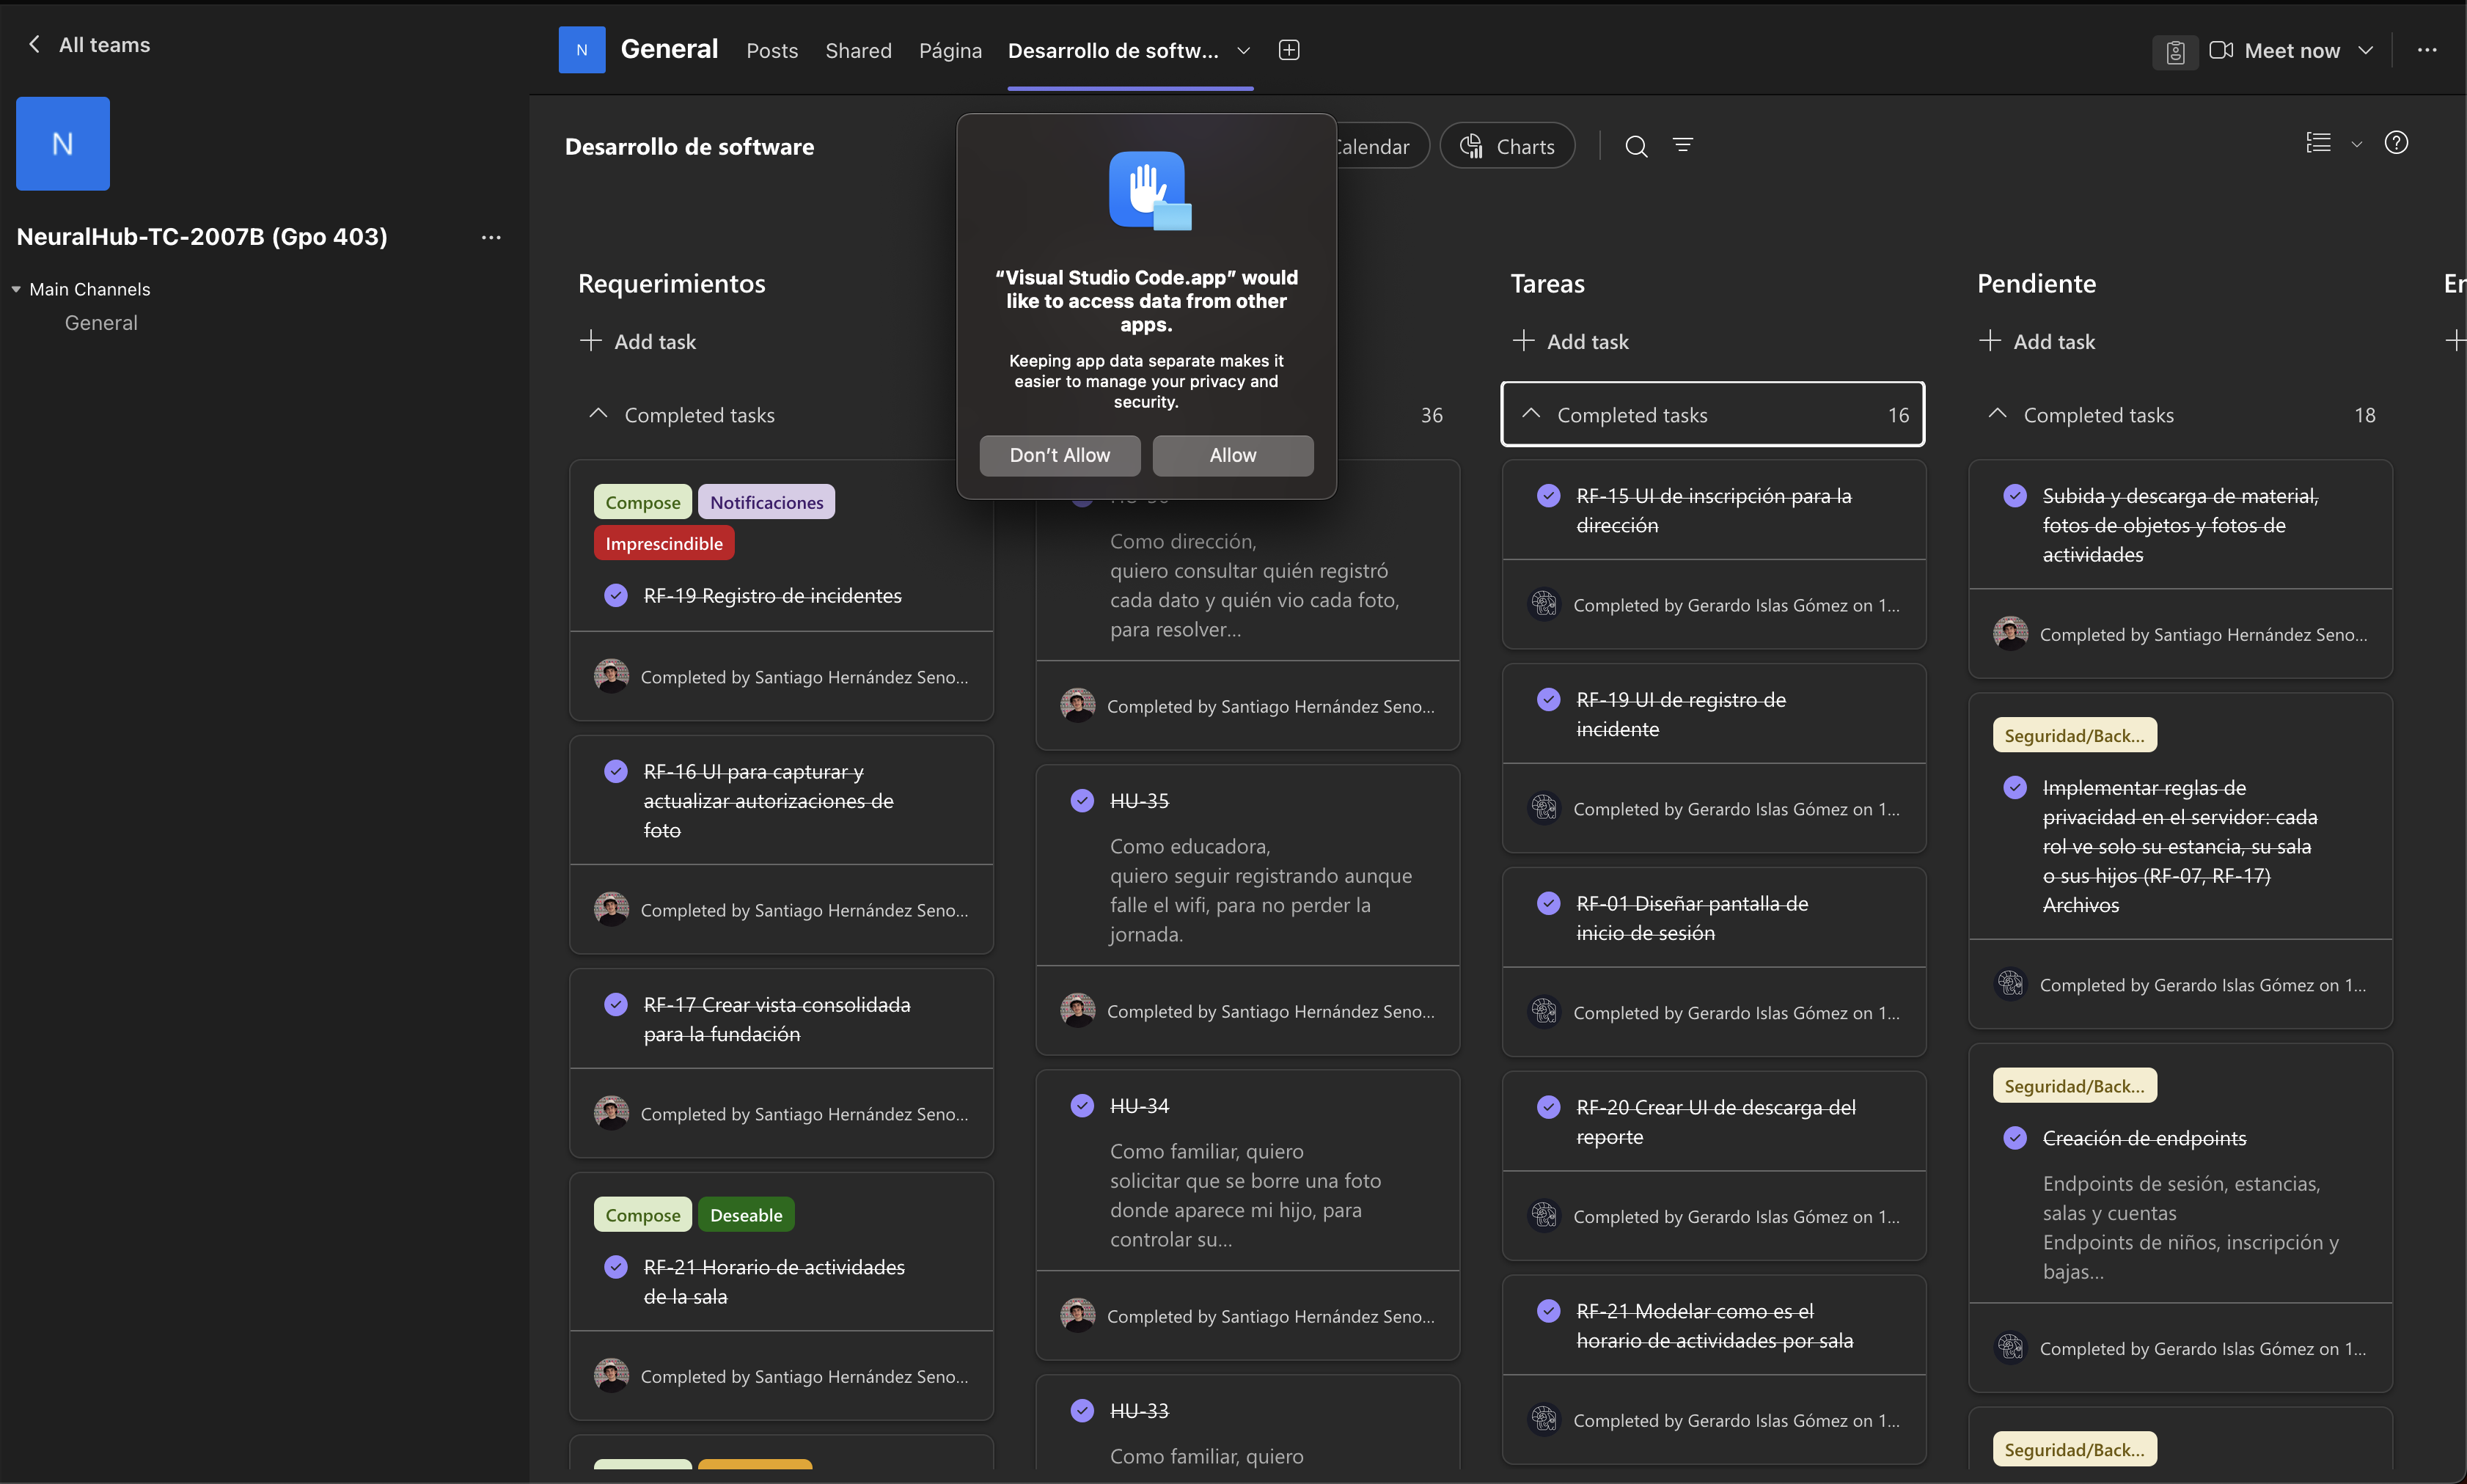
\includegraphics[width=\textwidth]{tablero-planner.png}
	\caption{Tablero final de Planner.}
\end{figure}

\subsection{Estado de los requerimientos}\label{sec:estado}
\begin{itemize}
	\item \textbf{Terminados (20):} RF-01 a RF-10 y RF-12 a RF-21, con la evidencia de la matriz de trazabilidad.
	\item \textbf{Fuera del alcance entregado (1):} RF-11, operación sin conexión. El backlog lo dejó abierto con preguntas sin resolver con el socio formador (qué acciones no deben permitirse sin conexión y qué dato gana en un conflicto), y no se comprometió su implementación. La app es solo en línea, y por eso el servidor puede ser la única fuente de verdad, incluida la hora.
	\item \textbf{Historias parciales:} HU-05, recuperar la contraseña sin la Dirección, no se implementó: las familias no usan correo de forma confiable. Hoy la Dirección genera una contraseña temporal nueva. El cambio obligatorio de contraseña en el primer acceso también queda pendiente.
\end{itemize}

\subsection{Bitácora de hitos}
\begin{longtable}{p{2.6cm}p{8.4cm}p{3.6cm}}
\toprule
\textbf{Fecha} & \textbf{Hito} & \textbf{Cumplimiento}\\\midrule\endhead
22 sep 2026 & Inicio del repositorio, arquitectura MVVM y módulo \texttt{shared/\allowbreak{}} & En fecha\\
Entrega 1 & Backlog con 21 RF, 8 épicas y 36 HU, validado con el socio formador; Presentación 1 & En fecha\\
2 oct 2026 & Entrega 2: prototipo funcional con datos en memoria & En fecha\\
3--14 oct 2026 & Backend Ktor + PostgreSQL e integración de la app con el API & En fecha\\
19--20 oct 2026 & Endurecimiento de seguridad P1--P8 y rediseño de UI (PR \#2 y \#3) & En fecha\\
21 oct 2026 & Pruebas por RF y pulido para la demostración & En fecha\\
22 oct 2026 & Entrega final: bloqueo multi-IP, archivos, hora del servidor, aviso de privacidad, borrado ARCO, ZAP y APK firmado & En fecha, con RF-11 fuera\\
\bottomrule
\end{longtable}

\subsection{Desviaciones}
\begin{itemize}
	\item \textbf{RF-11 (sin conexión) no se implementó.} Causa: el backend propio y la seguridad del API consumieron el tiempo previsto, y las reglas de conflicto nunca se definieron con el socio formador.
	\item \textbf{Los datos de demostración pasaron de la app a la base.} En la Entrega 2 la app usaba datos en memoria. En la final, la versión release solo consume el API, y la demostración vive en PostgreSQL mediante una semilla idempotente.
	\item \textbf{El trabajo se concentró al final.} La seguridad y la documentación se cerraron en los últimos días. Ver la retrospectiva.
\end{itemize}

\subsection{Riesgos}
\begin{longtable}{p{4.8cm}p{5.6cm}p{4.4cm}}
\toprule
\textbf{Riesgo} & \textbf{Acción tomada} & \textbf{Resultado}\\\midrule\endhead
Fuga de fotos o datos de menores & Autorización por objeto en el servidor, permisos de imagen y limpieza de metadatos & Mitigado; pruebas RF07, RF09, SEG y ARCO\\
Red del campus bloquea el túnel (QUIC) & \texttt{cloudflared} con HTTP/2 sobre TCP 443 & Resuelto\\
Fuerza bruta contra cuentas & Rate limiting y bloqueo por cuenta y multi-IP & Mitigado; S15--S19\\
Servidor caído durante la presentación & Video de respaldo y servidor local con emulador & Plan de contingencia listo\\
Dirección del túnel rápido cambia & Configuración del servidor en la app (mantener presionado el logo) & Aceptado; en producción, túnel con nombre\\
Datos inconsistentes entre teléfonos con relojes distintos & Hora del servidor como autoridad & Resuelto; \texttt{SEGReloj\allowbreak{}Servidor\allowbreak{}Test}\\
\bottomrule
\end{longtable}

\subsection{Distribución del trabajo}
La evidencia está en el historial de \texttt{git} (autores de los commits y pull requests) y en las asignaciones de Planner.
\begin{itemize}
	\item \textbf{Santiago Hernández Senosiain:} arquitectura, app Android, backend Ktor, integración, controles de seguridad finales, pruebas y documentación de la entrega final.
	\item \textbf{Gilberto Olavarrieta Sánchez:} rediseño de la interfaz de todas las pantallas por rol (PR \#3, \texttt{rediseno-ui}).
	\item \textbf{Franco Salazar Guerrero:} borradores del reporte de entregas y documentación de avance.
	\item \textbf{Gerardo Islas Gómez:} endurecimiento de seguridad P1--P8: cabeceras, contraseñas temporales, token cifrado en el teléfono, Docker endurecido, secretos en \texttt{.\allowbreak{}env} y túnel HTTPS (PR \#2, \texttt{seguridad}).
\end{itemize}

\subsection{Retrospectiva}
\begin{description}
	\item[Qué funcionó.]
	\begin{itemize}
		\item Compartir el módulo \texttt{shared/\allowbreak{}} entre la app y el servidor. La regla «cada familia ve solo a sus hijos» se escribió una vez y se probó una vez.
		\item Nombrar las pruebas por RF. La matriz de trazabilidad salió casi sola de los nombres de las clases de prueba.
		\item Ponerle número a cada cambio de seguridad (P1--P8) y dejarlo en el commit, lo que hizo fácil explicar cada control.
	\end{itemize}
	\item[Qué no funcionó.]
	\begin{itemize}
		\item Construir el prototipo con datos en memoria en la app (Entrega 2) obligó a mantener dos implementaciones de cada repositorio, la falsa y la remota, hasta el final.
		\item Varios huecos se descubrieron hasta la auditoría final: imágenes que quedaban huérfanas al borrar un expediente y fechas que mandaba el cliente.
		\item El trabajo de seguridad y documentación quedó concentrado en los últimos días, y la distribución entre integrantes fue desigual.
	\end{itemize}
	\item[Qué cambiaríamos.]
	\begin{itemize}
		\item Levantar el backend mínimo desde el Sprint 1 y escribir el aviso de privacidad desde el inicio, para diseñar el borrado de datos junto con el modelo y no al final.
		\item Asignar en Planner a cada integrante un módulo con pruebas propias desde la primera semana, para que la contribución quede visible en \texttt{git} y no dependa de una sola persona.
		\item Cerrar con el socio formador las preguntas abiertas del backlog, por ejemplo las de RF-11, antes de comprometer el alcance.
	\end{itemize}
\end{description}
